\documentclass{beamer}
\usepackage[utf8]{inputenc}
\usepackage{amssymb}
\usepackage{xcolor}

\title[Nelder-Mead on the Rheology Problem]{Chapter 5 Project: Apply Nelder-Mead to the Rheology Problem}
\author[Matthew, Tyler, and Sarah]{Matthew Saurette, Tyler ``can put his hand in his mouth" Weames, and Sarah Wyse}
\institute[Math 462]{Math 462\\ University of British Columbia - Okanagan}
\date{December 2020}
\usetheme{Madrid}
\usecolortheme{seahorse} 
\useinnertheme{rounded}

\begin{document}
\maketitle


%%%%The Rheology Problem
%------------------------------------------------------------------------
\begin{frame}{The Rheology Problem}
\begin{block}{Viscosity of a system}
$$\eta(\dot{\gamma}) = \eta_0(1+\lambda^2\dot{\gamma}^2)^{\frac{\beta -1}{2}}$$
A function of the strain rate, $\dot{\gamma}$, with parameters $\eta_0$, $\lambda$, and $\beta$.
\end{block}
\begin{columns}
	\begin{column}{0.45\linewidth}
		\centering
		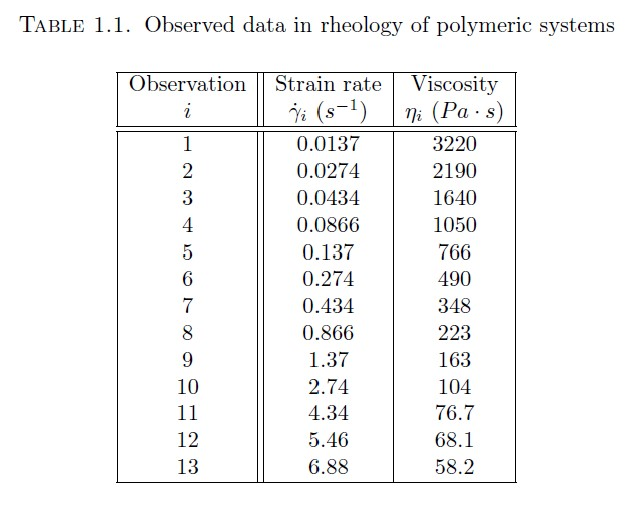
\includegraphics[width=0.95\linewidth]{Data}
	\end{column}
	\begin{column}{0.53\linewidth}
		Absolute Error:
		$$\epsilon_i(\eta_0, \lambda, \beta) = |\eta_0(1+\lambda^2\dot{\gamma}^2)^{\frac{\beta -1}{2}} - \eta_i|$$
		Non-smooth optimization problem:
		$$\hat{g}(\eta_0, \lambda, \beta) = \sum\limits_{i=1}^{13}\epsilon_i(\eta_0, \lambda, \beta)$$
	\end{column}
\end{columns}
\hfill \tiny (Audet and Hare, 2017)
\end{frame}

%%%%The NM Algorithm
%-------------------------------------------------------------------------
\begin{frame}{Nelder-Mead Algorithm}
    \centering
    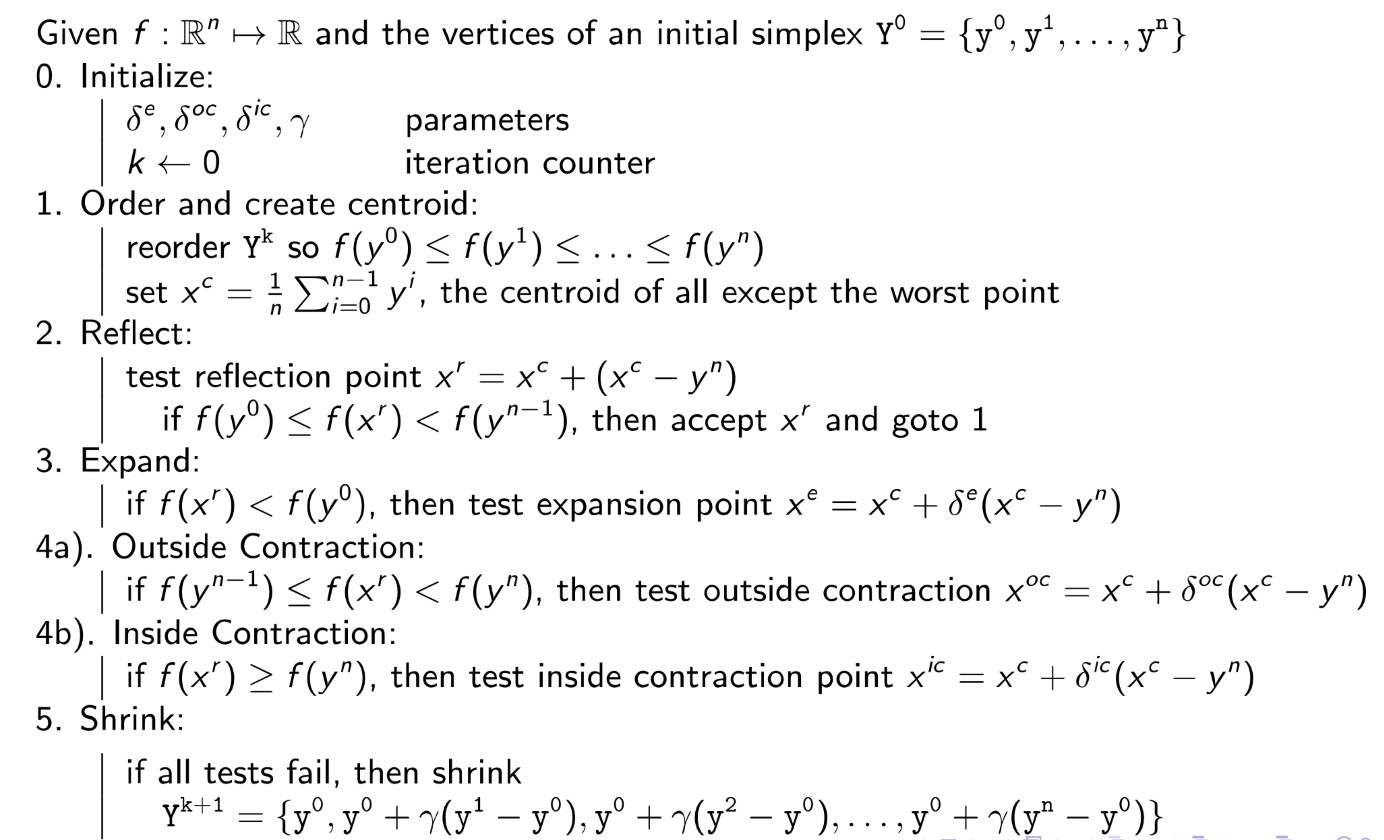
\includegraphics[width=0.95\linewidth]{NMAlgorithm}\\
	\hfill \tiny (Math 462, UBCO, 2020) 
\end{frame}

\begin{frame}{0. Initialize}
	\centering
	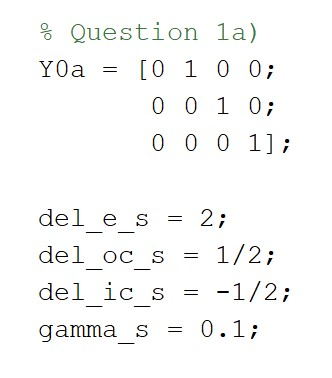
\includegraphics[width=0.35\linewidth]{Initialize}
	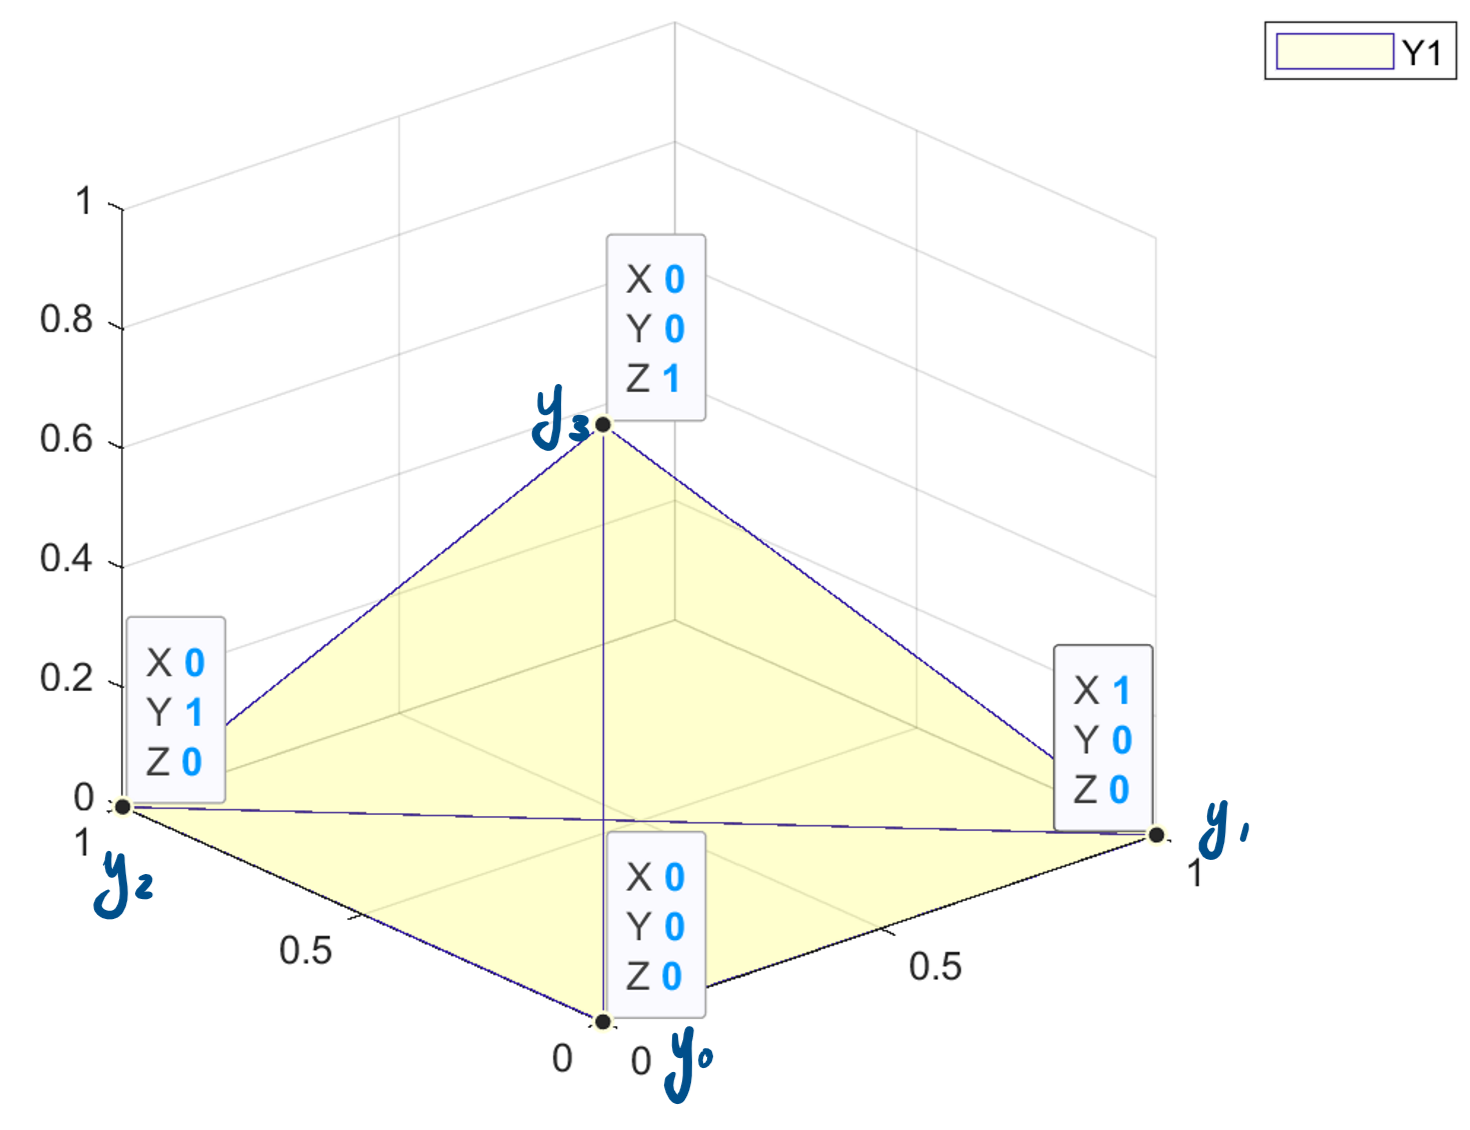
\includegraphics[width=0.59\linewidth]{InitializeFig}
\end{frame}

\begin{frame}{1. Order}
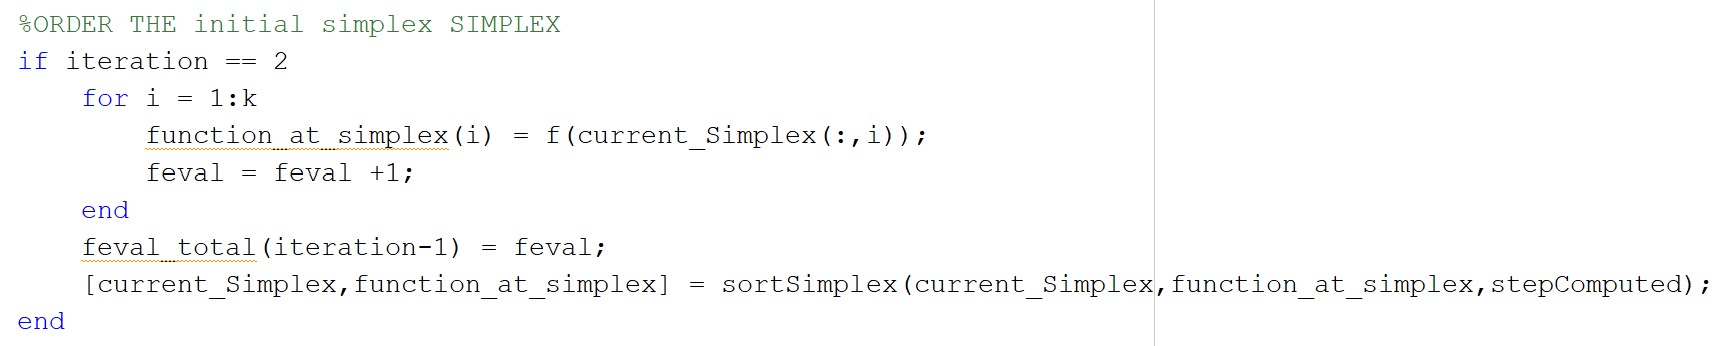
\includegraphics[width=0.75\linewidth]{Order1}
	\begin{columns}
	\begin{column}{0.35\linewidth}
		\centering
		
		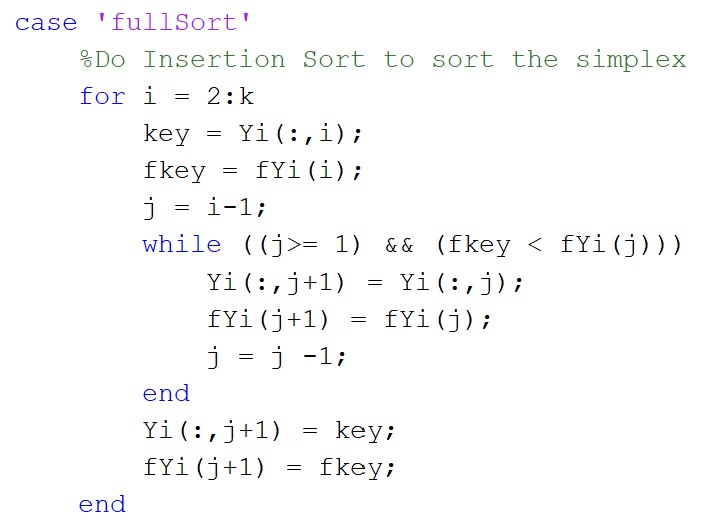
\includegraphics[width=0.95\linewidth]{Shrink2}
		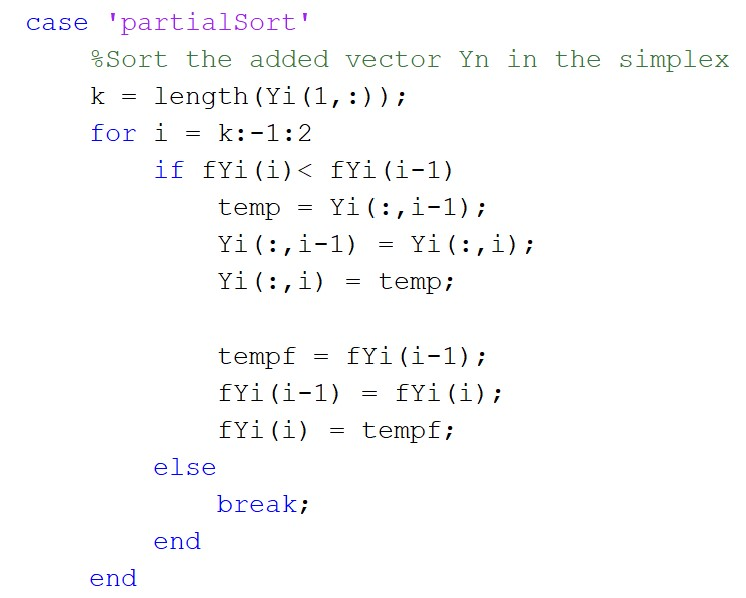
\includegraphics[width=0.95\linewidth]{Order3}
	\end{column}
	\begin{column}{0.59\linewidth}
		\centering
		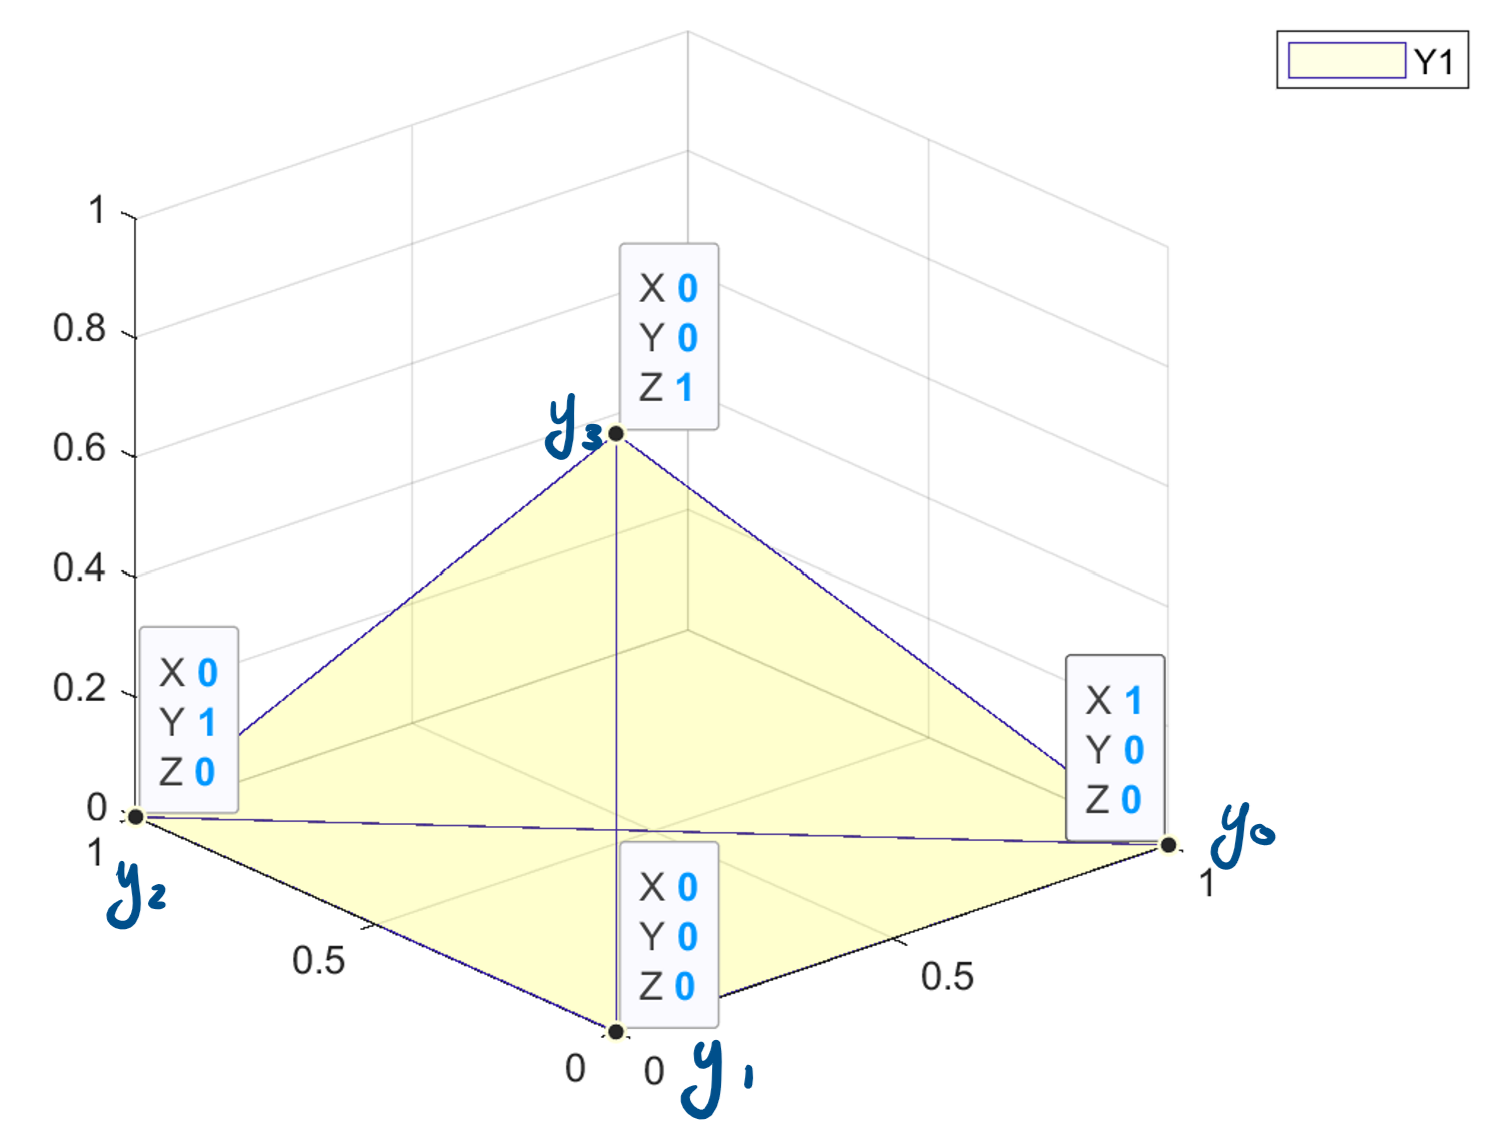
\includegraphics[width=0.95\linewidth]{Order1Fig}
	\end{column}
	\end{columns}
\end{frame}

\begin{frame}{1 and 2. Calculate centroid and $x^r$}
	\begin{columns}
	\begin{column}{0.35\linewidth}
		\centering
		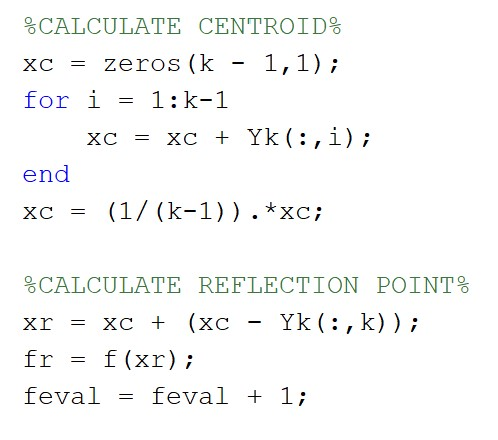
\includegraphics[width=0.95\linewidth]{Order2}
	\end{column}
	\begin{column}{0.59\linewidth}
		\centering
		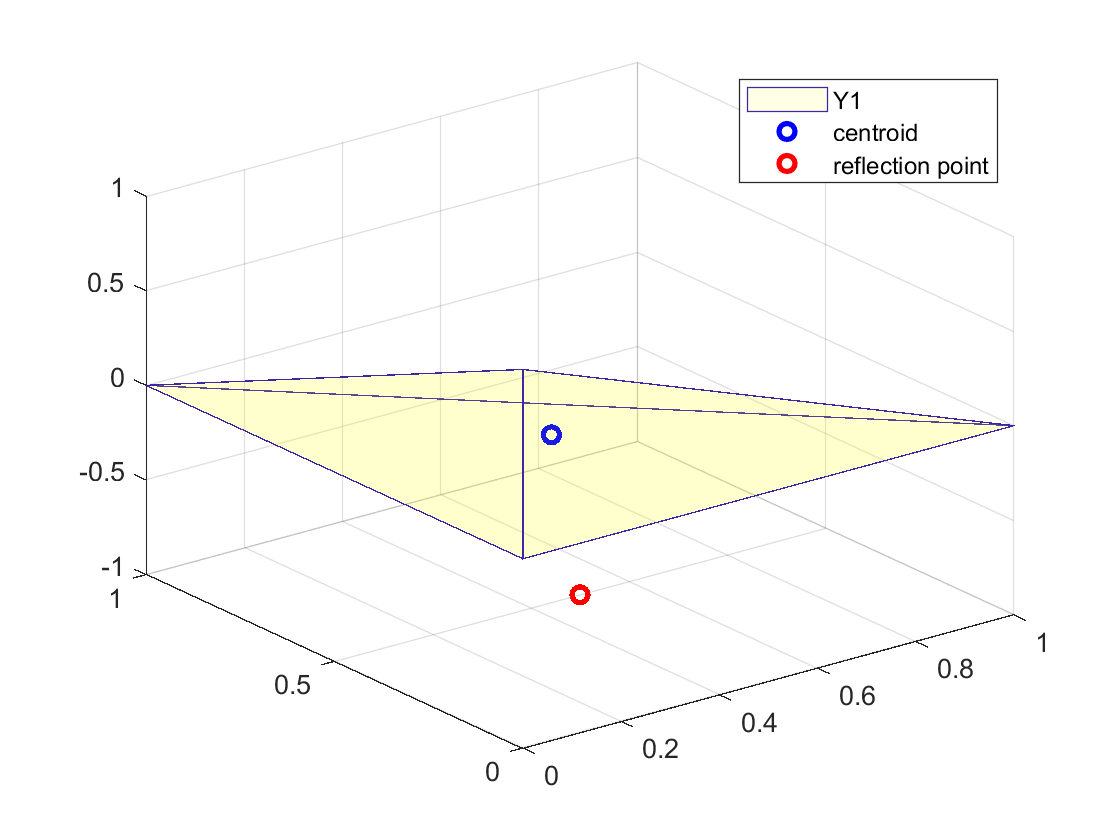
\includegraphics[width=0.95\linewidth]{Order2Fig}
	\end{column}
	\end{columns}
\end{frame}

\begin{frame}{2. Reflect}
	\begin{columns}
	\begin{column}{0.39\linewidth}
		\centering
		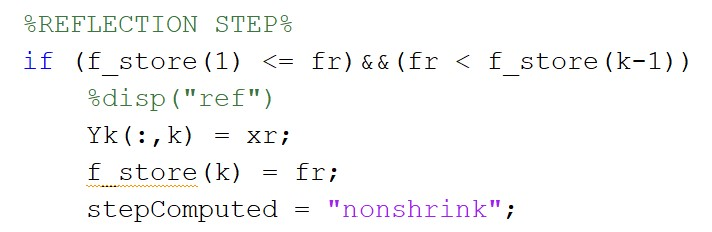
\includegraphics[width=0.95\linewidth]{Reflect}
	\end{column}
	\begin{column}{0.59\linewidth}
		\centering
		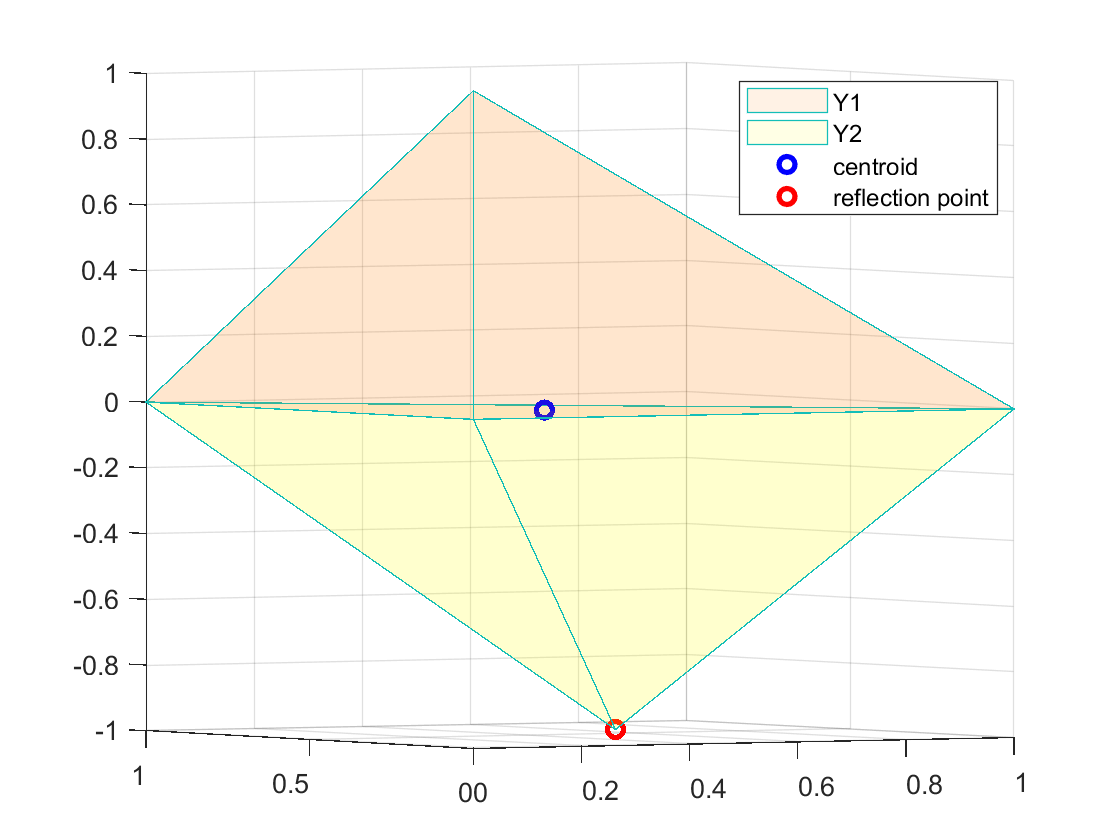
\includegraphics[width=0.95\linewidth]{ReflectFig}
	\end{column}
	\end{columns}
\end{frame}

\begin{frame}{3. Expand}
	\begin{columns}
	\begin{column}{0.39\linewidth}
		\centering
		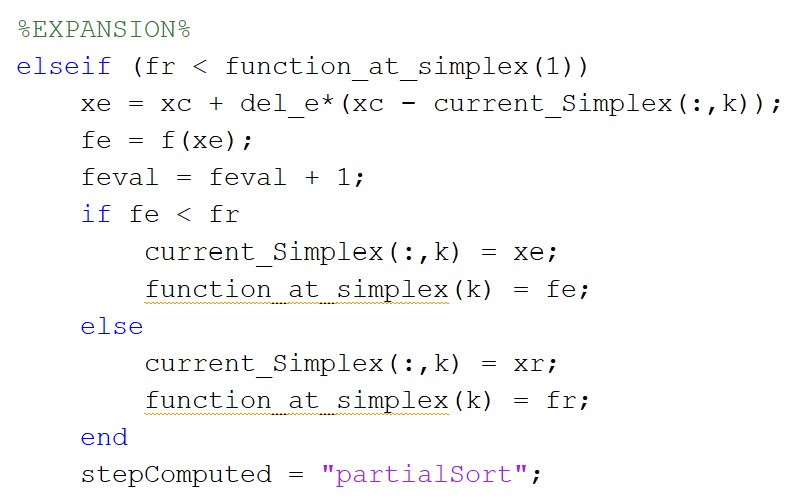
\includegraphics[width=0.95\linewidth]{Expand}
	\end{column}
	\begin{column}{0.59\linewidth}
		\centering
		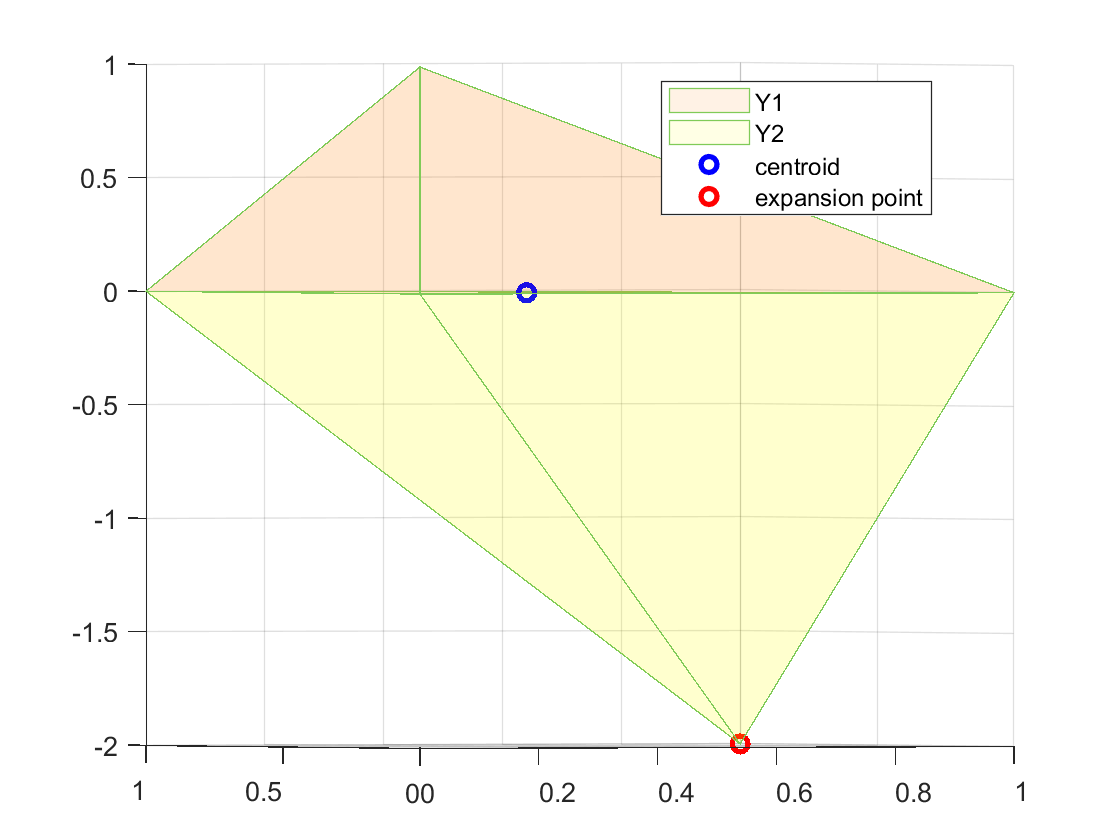
\includegraphics[width=0.95\linewidth]{ExpandFig}
	\end{column}
	\end{columns}
\end{frame}

\begin{frame}{4.a) Outside Contraction}
	\begin{columns}
	\begin{column}{0.39\linewidth}
		\centering
		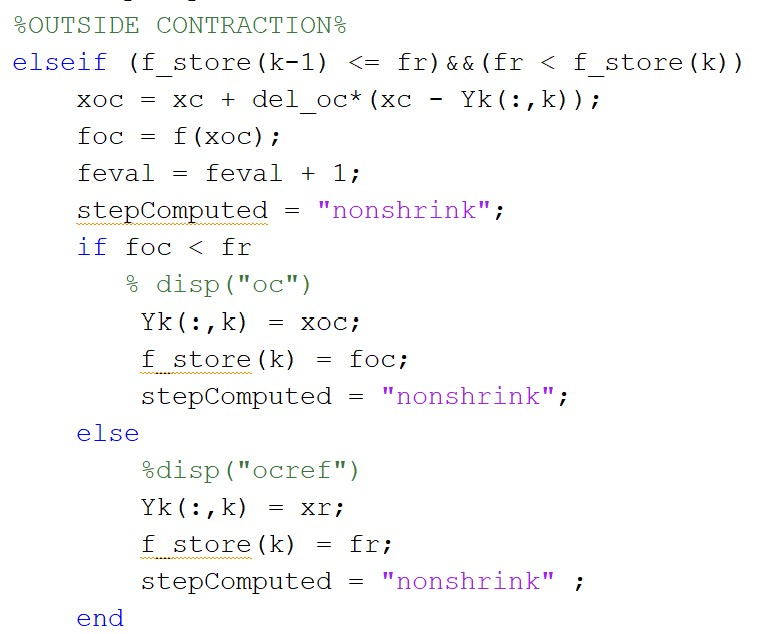
\includegraphics[width=0.95\linewidth]{OC}
	\end{column}
	\begin{column}{0.59\linewidth}
		\centering
		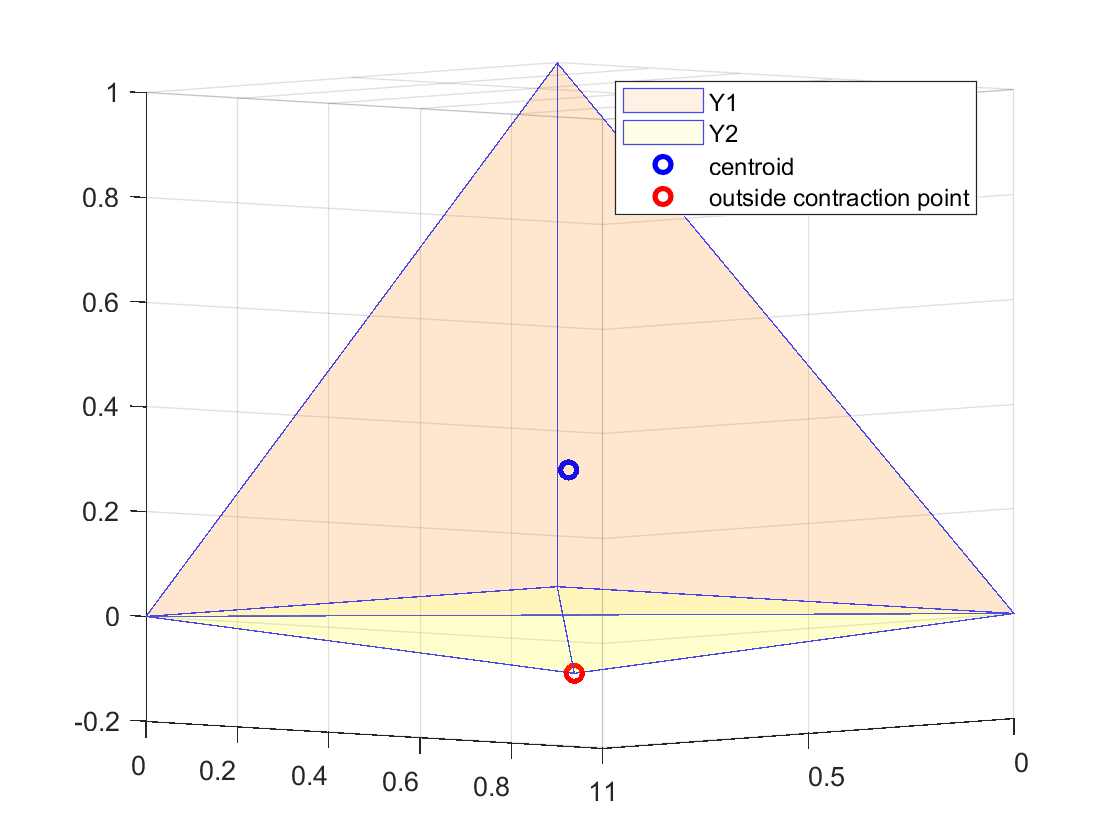
\includegraphics[width=0.95\linewidth]{OCFig}
	\end{column}
	\end{columns}
\end{frame}

\begin{frame}{4.b) Inside Contraction}
	\begin{columns}
	\begin{column}{0.39\linewidth}
		\centering
		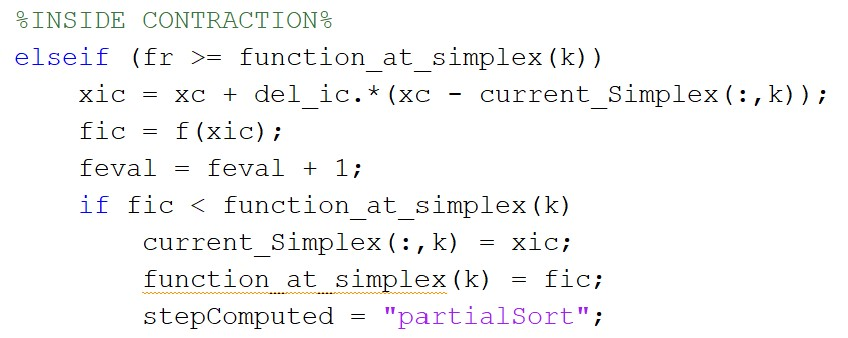
\includegraphics[width=0.95\linewidth]{IC}
	\end{column}
	\begin{column}{0.59\linewidth}
		\centering
		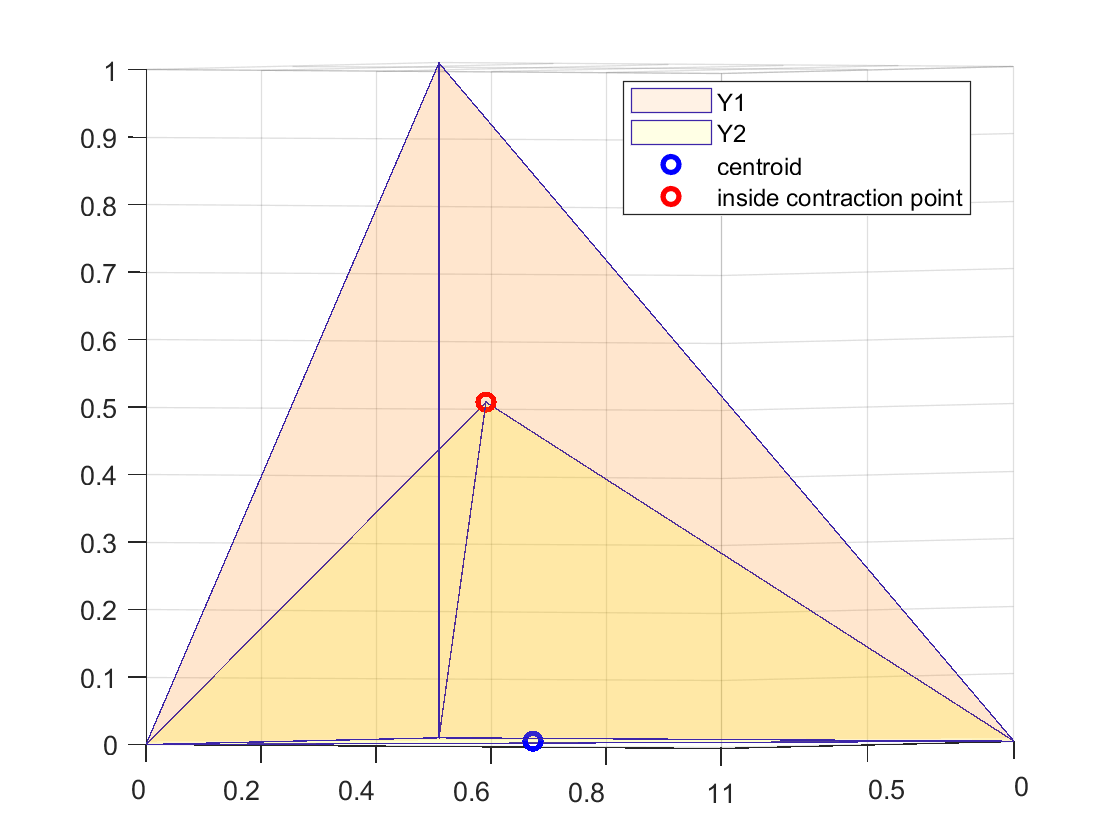
\includegraphics[width=0.95\linewidth]{ICFig}
	\end{column}
	\end{columns}
\end{frame}

\begin{frame}{5. Shrink}
	\begin{columns}
	\begin{column}{0.39\linewidth}
		\centering
		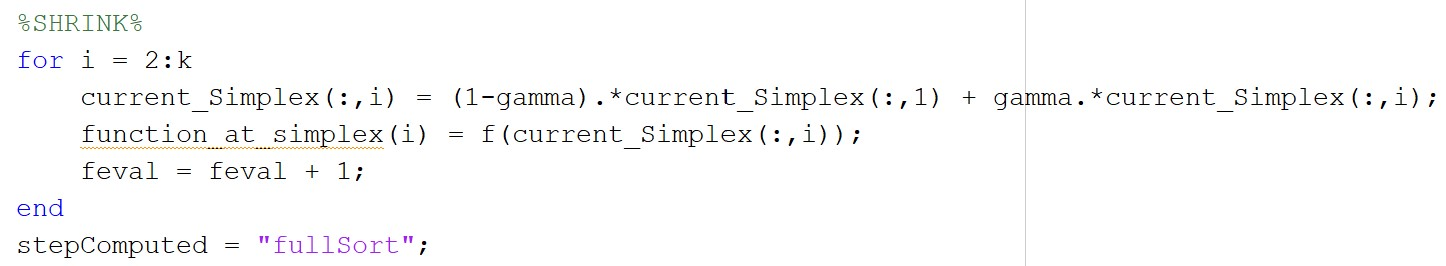
\includegraphics[width=0.95\linewidth]{Shrink}
		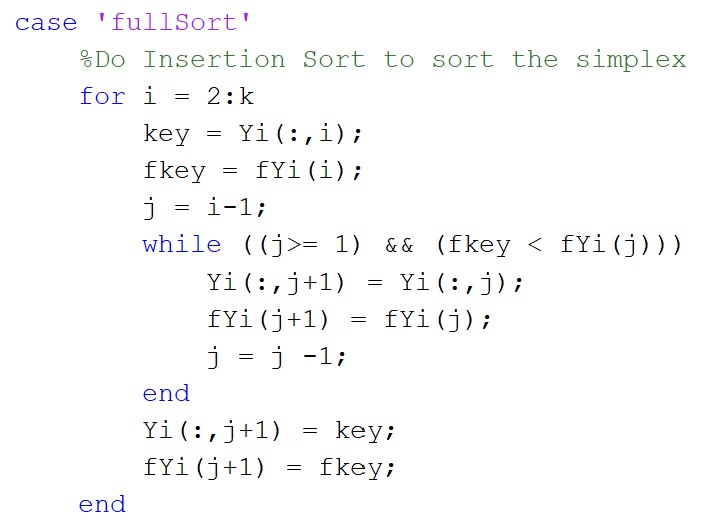
\includegraphics[width=0.85\linewidth]{Shrink2}
	\end{column}
	\begin{column}{0.59\linewidth}
		\centering
		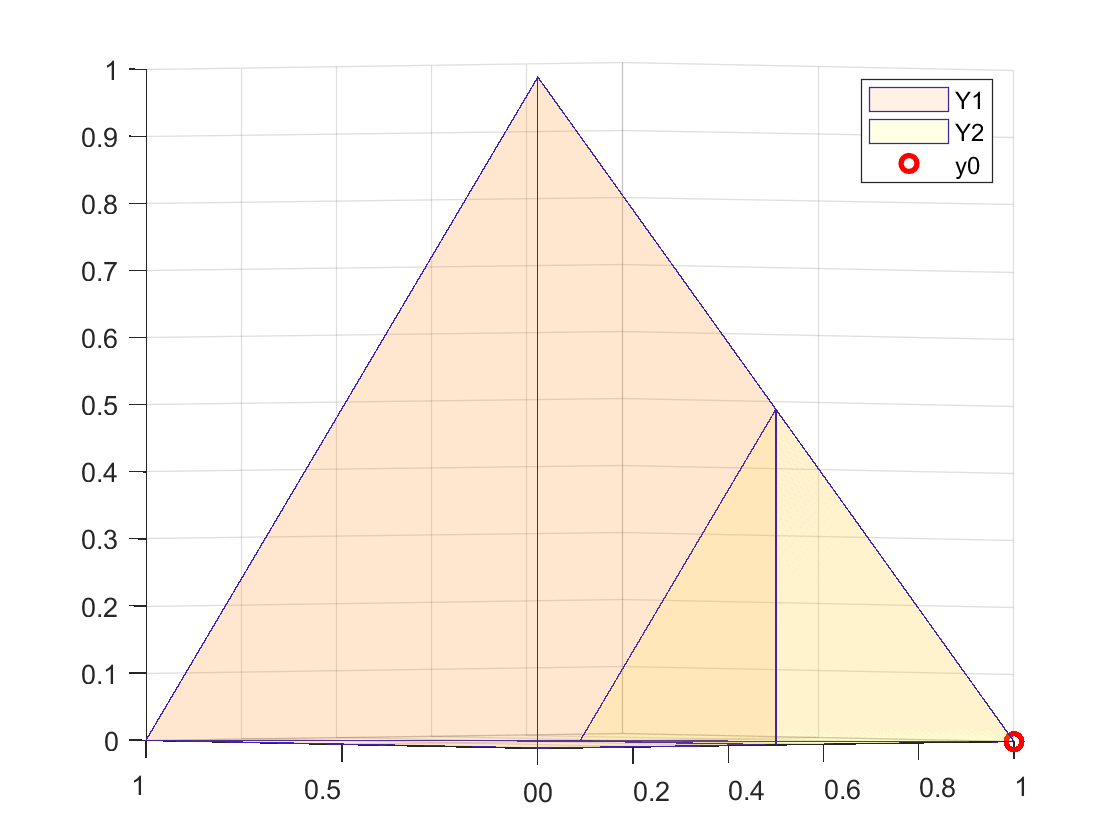
\includegraphics[width=0.95\linewidth]{ShrinkFig}
	\end{column}
	\end{columns}
\end{frame}

%%%%Examples
%------------------------------------------------------------------------
\begin{frame}{Examples of Nelder-Mead at work: A nice example}
\begin{columns}
\begin{column}{0.49\linewidth}
	$$f(x) = x_1^2 + x_2^2 - 2$$
	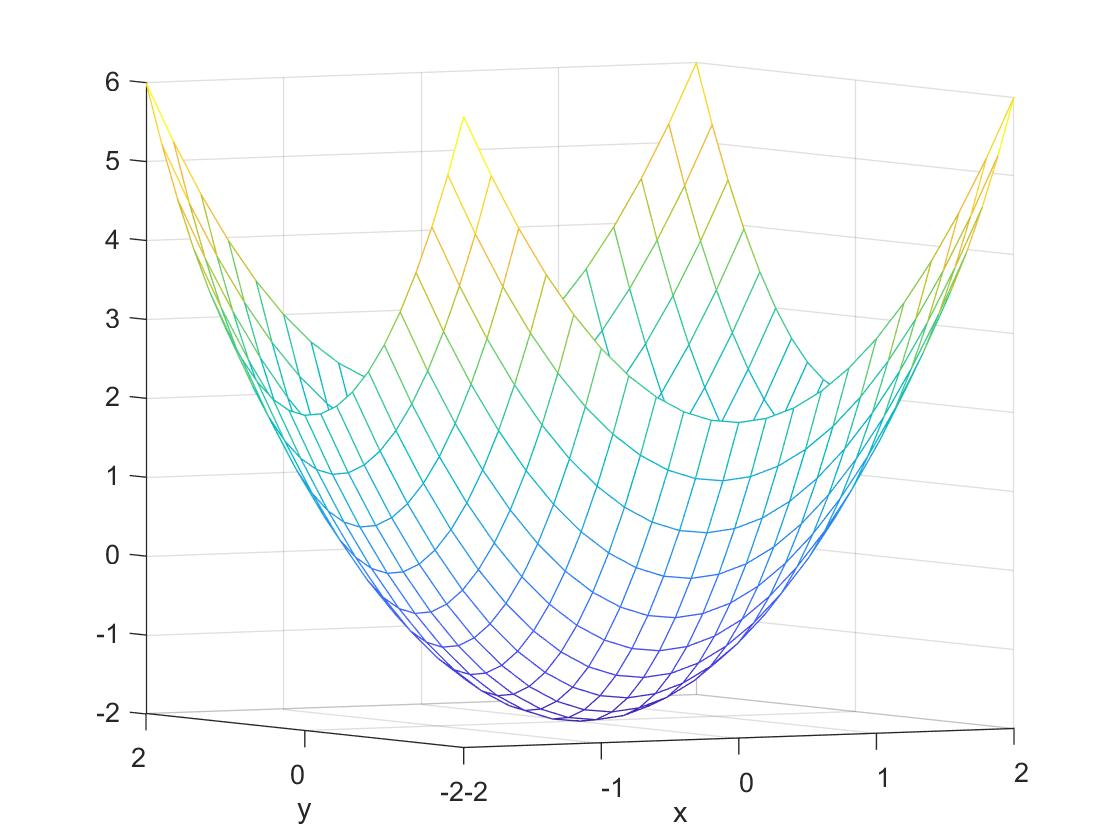
\includegraphics[width=0.95\linewidth]{NiceFunctionPlot}	\\
	$min(f(x))=-2$ for $x=(0,0)$
\end{column}
\begin{column}{0.49\linewidth}
	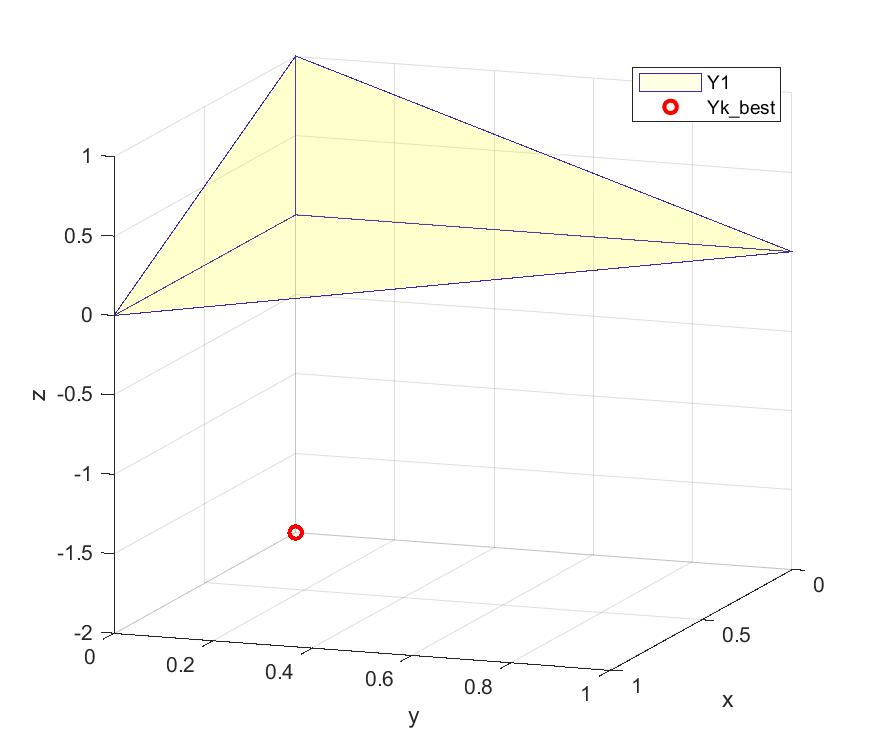
\includegraphics[width=0.95\linewidth]{NiceFunctionSimplex}	\\
	$f^k_{best}=-2$ for $x^k_{best}=(0,0)$
\end{column}
\end{columns}
\end{frame}

\begin{frame}{Examples of Nelder-Mead at work: Rosenbrock function}
\begin{columns}
\begin{column}{0.49\linewidth}
	$f(x) =(1-x_1)^2 + 100(x_2-x_1)^2$ \\
	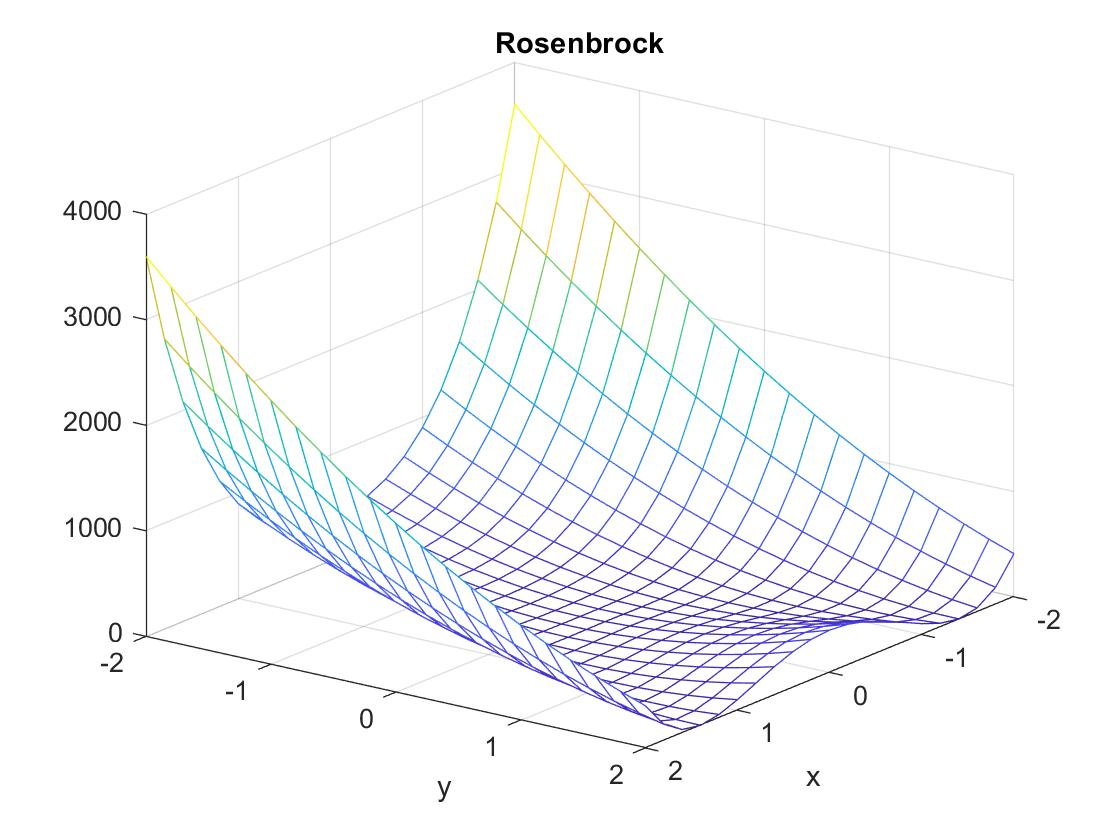
\includegraphics[width=0.95\linewidth]{rosenbrockPlotS1} \\
	$min(f(x))= fill in here $ for $x= fill in here$
\end{column}
\begin{column}{0.49\linewidth}
	put initial simplex and resulting simplex here\\
	$f^k_{best}= fill in here $ for $x^k_{best}= fill in here$
\end{column}
\end{columns}
\end{frame}

\begin{frame}{Examples of Nelder-Mead at work: Rastrigin function}
\begin{columns}
\begin{column}{0.49\linewidth}
	\small $f(x) = 20 + x_1^2 - 10cos(2\pi x_1) + x_2^2 - 10cos(2\pi x_2)$ \\
	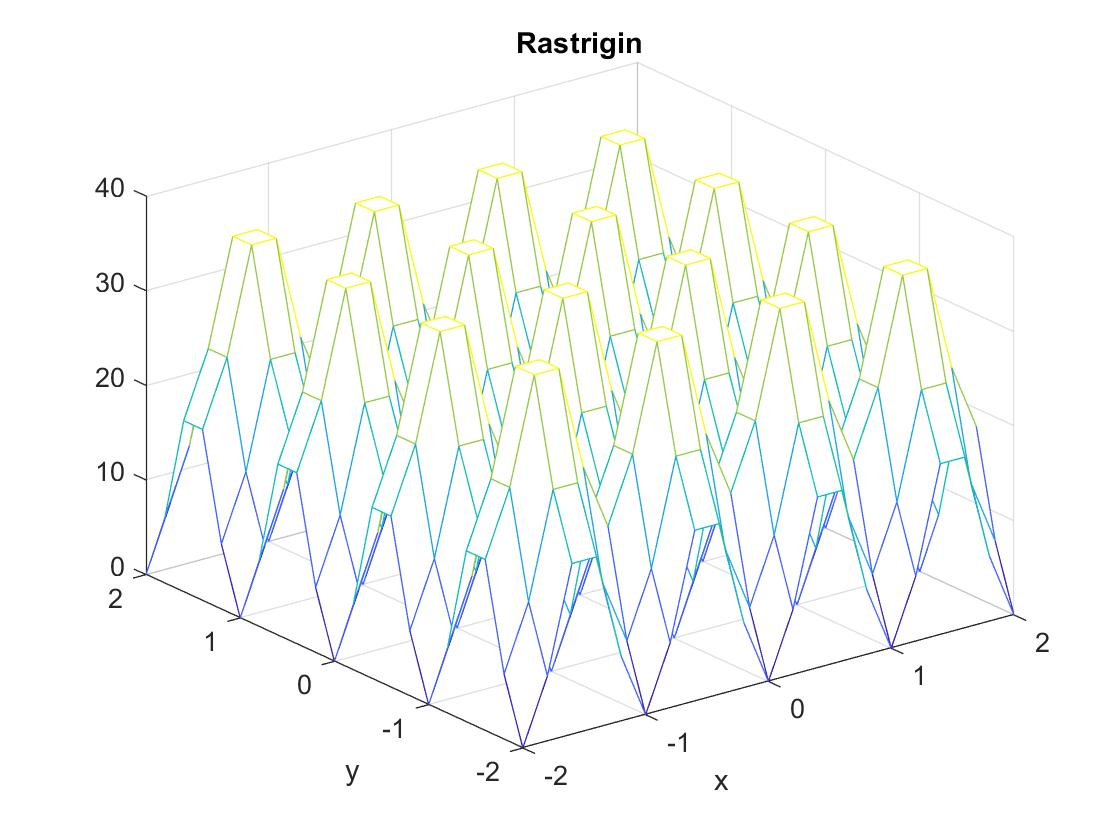
\includegraphics[width=0.95\linewidth]{rastriginPlotS1}	 \\
	$min(f(x))= fill in here $ for $x= fill in here$
\end{column}
\begin{column}{0.49\linewidth}
	put initial simplex and resulting simplex here\\
	$f^k_{best}= fill in here $ for $x^k_{best}= fill in here$
\end{column}
\end{columns}
\end{frame}

\begin{frame}{Examples of Nelder-Mead at work: Rastrigin function}
\begin{columns}
\begin{column}{0.49\linewidth}
	\small $f(x) = 20 + x_1^2 - 10cos(2\pi x_1) + x_2^2 - 10cos(2\pi x_2)$ \\
	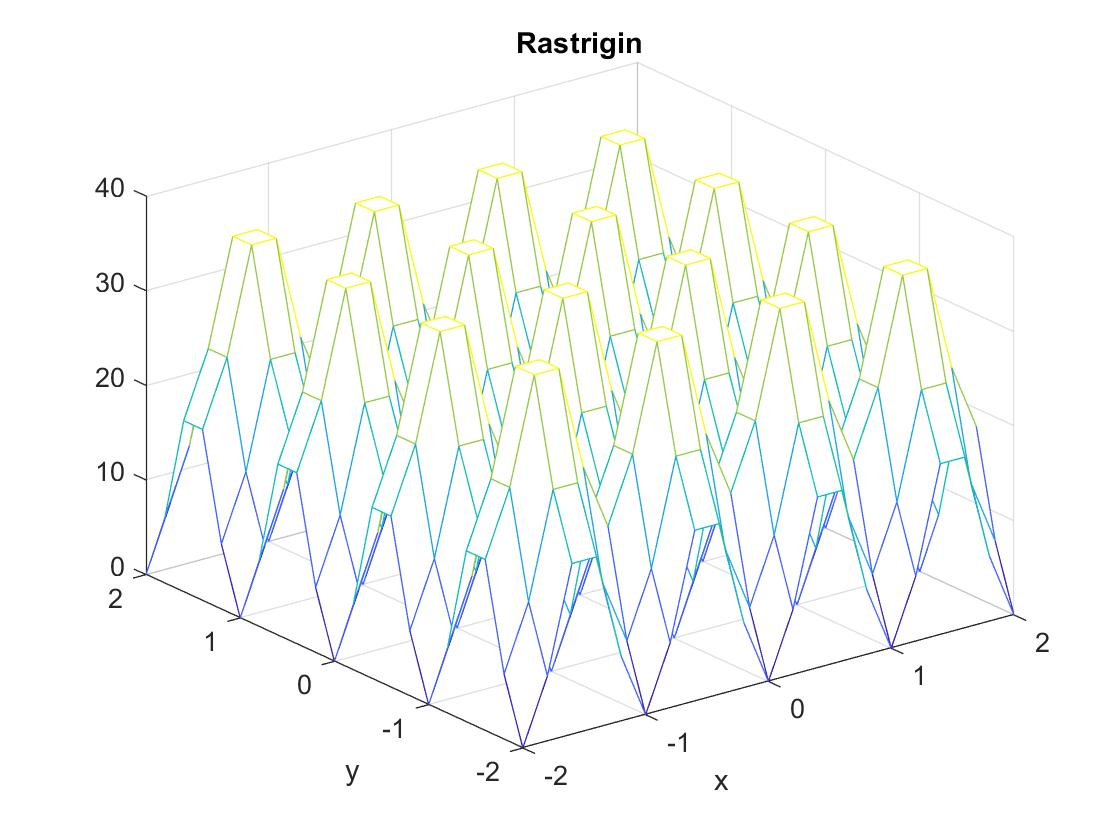
\includegraphics[width=0.95\linewidth]{rastriginPlotS1}	\\
	$min(f(x))= fill in here $ for $x= fill in here$
\end{column}
\begin{column}{0.49\linewidth}
	use a different starting simplex to get a different min that still minimizes \\
	put initial simplex and resulting simplex here \\
	$f^k_{best}= fill in here $ for $x^k_{best}= fill in here$
\end{column}
\end{columns}
\end{frame}


%%%%Solve the Rheology Problem
%------------------------------------------------------------------------
\begin{frame}{The Rheology Problem: Solved}
\begin{block}{1.a) Standard parameters with simplex A}
\begin{columns}
\begin{column}{0.35\linewidth}
	\underline{Input:}\\
	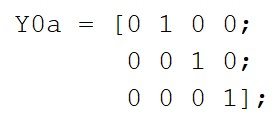
\includegraphics[width=0.45\linewidth]{Y0a}\\
	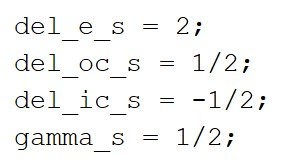
\includegraphics[width=0.45\linewidth]{StandardParams}\\
	\vspace{0.65cm}
	\underline{Output:}\\
	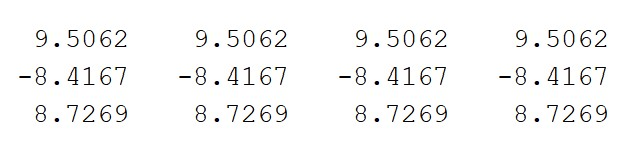
\includegraphics[width=0.95\linewidth]{1aSimplex}
	$$f^k_{best} = 32.7239$$
	\vspace{0.1cm}
\end{column}
\begin{column}{0.63\linewidth}
	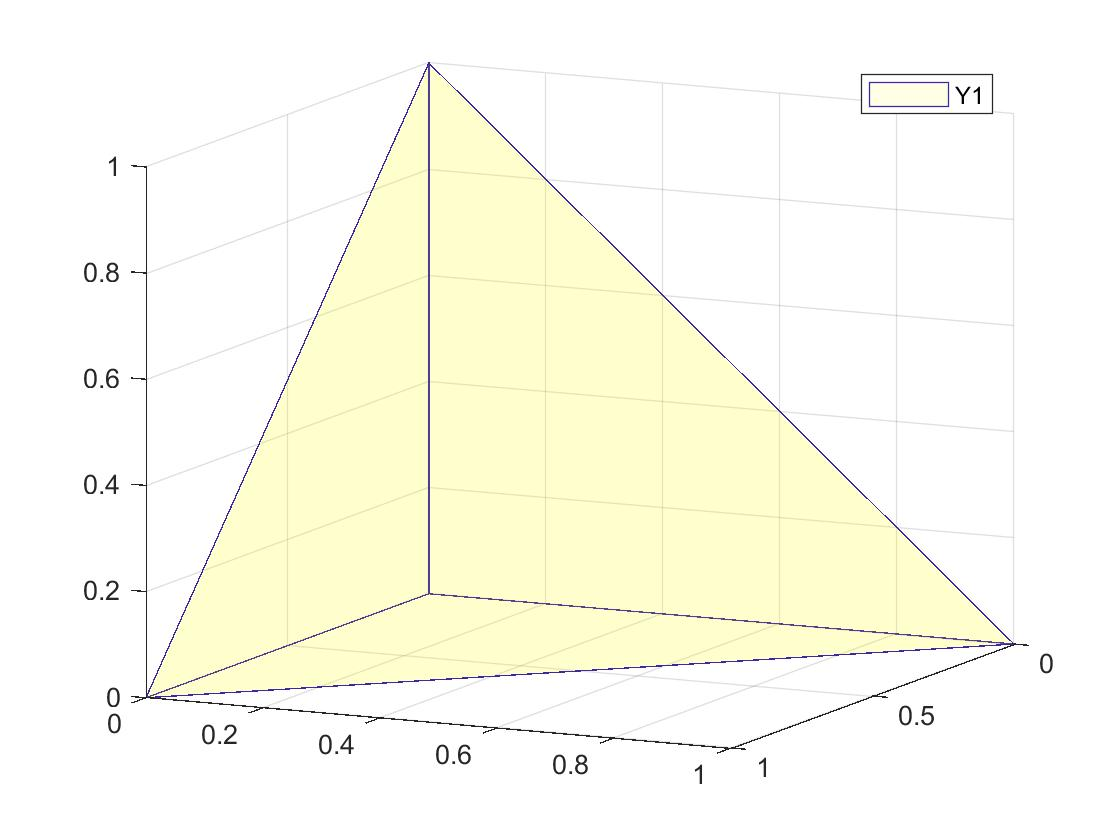
\includegraphics[width=0.45\linewidth]{Simplex1}\\
	\vspace{5mm}
	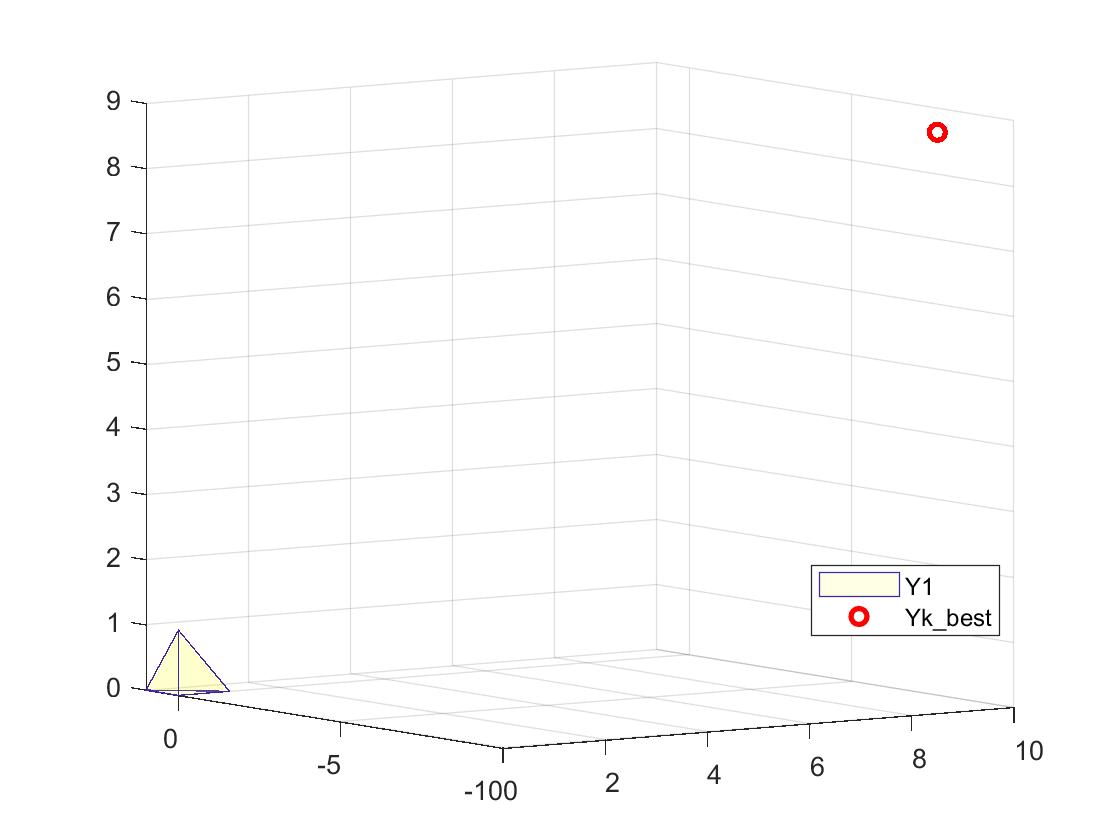
\includegraphics[width=0.45\linewidth]{1aSimplexPlot}
\end{column}
\end{columns}
\end{block}
\end{frame}

\begin{frame}{The Rheology Problem: Solved}
\begin{block}{1.b) Standard parameters with simplex B}
\begin{columns}
\begin{column}{0.35\linewidth}
	\underline{Input:}\\
	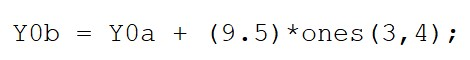
\includegraphics[width=0.75\linewidth]{Y0b}\\
	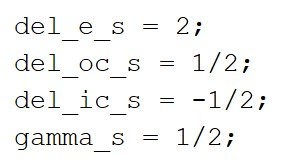
\includegraphics[width=0.45\linewidth]{StandardParams}\\
	\vspace{0.65cm}
	\underline{Output:}\\
	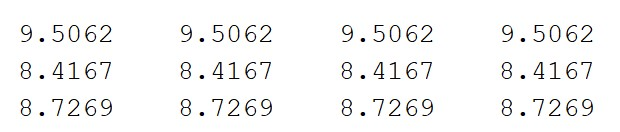
\includegraphics[width=0.95\linewidth]{1bSimplex}
	$$f^k_{best} = 32.7238$$
	\vspace{0.1cm}
\end{column}
\begin{column}{0.63\linewidth}
	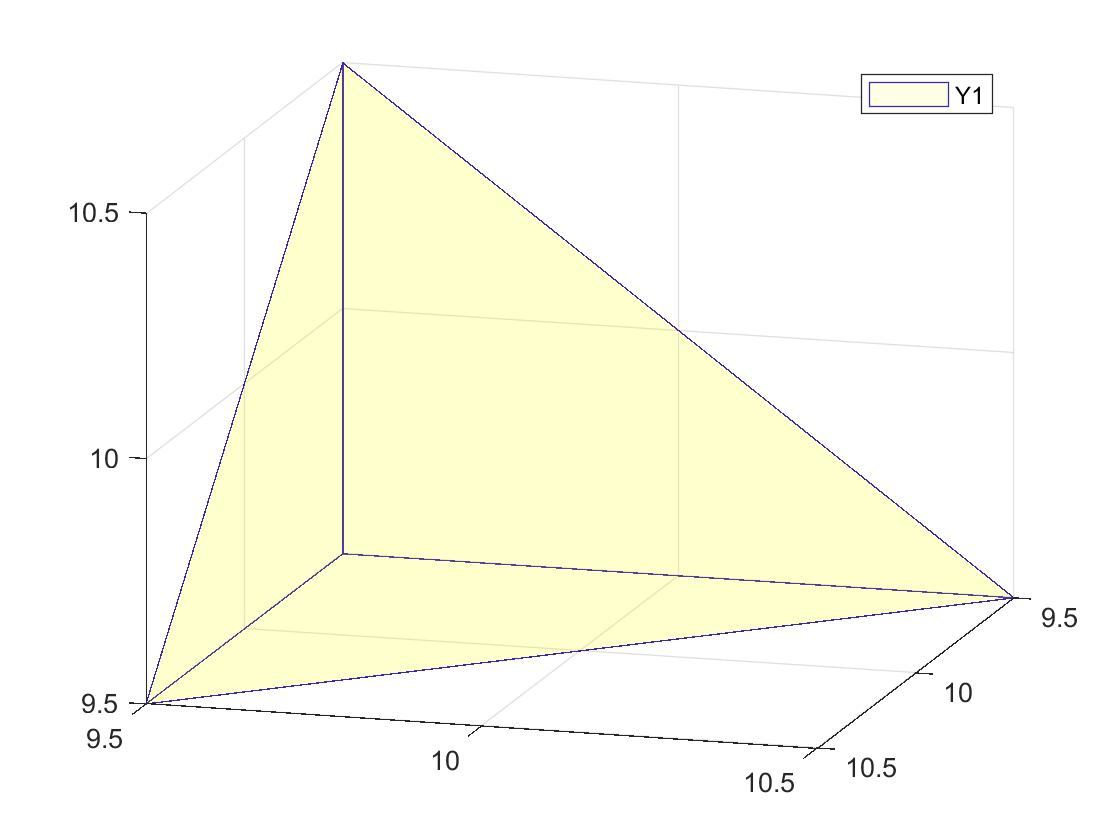
\includegraphics[width=0.45\linewidth]{Simplex2}\\
	\vspace{5mm}
	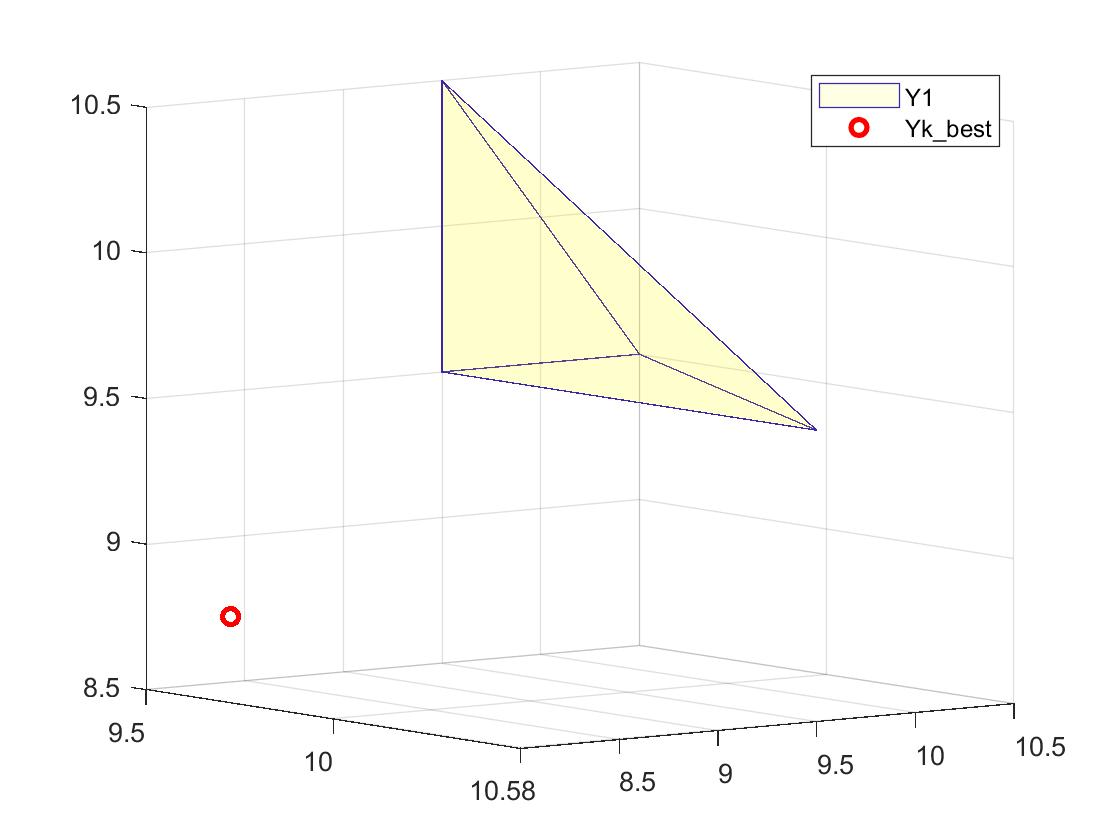
\includegraphics[width=0.45\linewidth]{1bSimplexPlot}
\end{column}
\end{columns}
\end{block}
\end{frame}

\begin{frame}{The Rheology Problem: Solved}
\begin{block}{2.a) New parameters with simplex A}
\begin{columns}
\begin{column}{0.35\linewidth}
	\underline{Input:}\\
	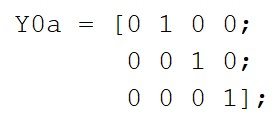
\includegraphics[width=0.45\linewidth]{Y0a}\\
	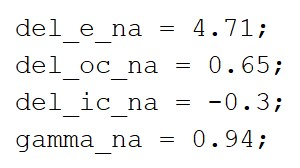
\includegraphics[width=0.45\linewidth]{NewParamsA}\\
	\vspace{0.65cm}
	\underline{Output:}\\
	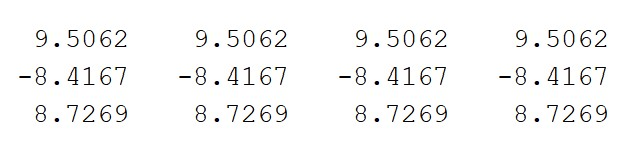
\includegraphics[width=0.95\linewidth]{1aSimplex}
	$$f^k_{best} = 32.7238$$
	\vspace{0.1cm}
\end{column}
\begin{column}{0.63\linewidth}
	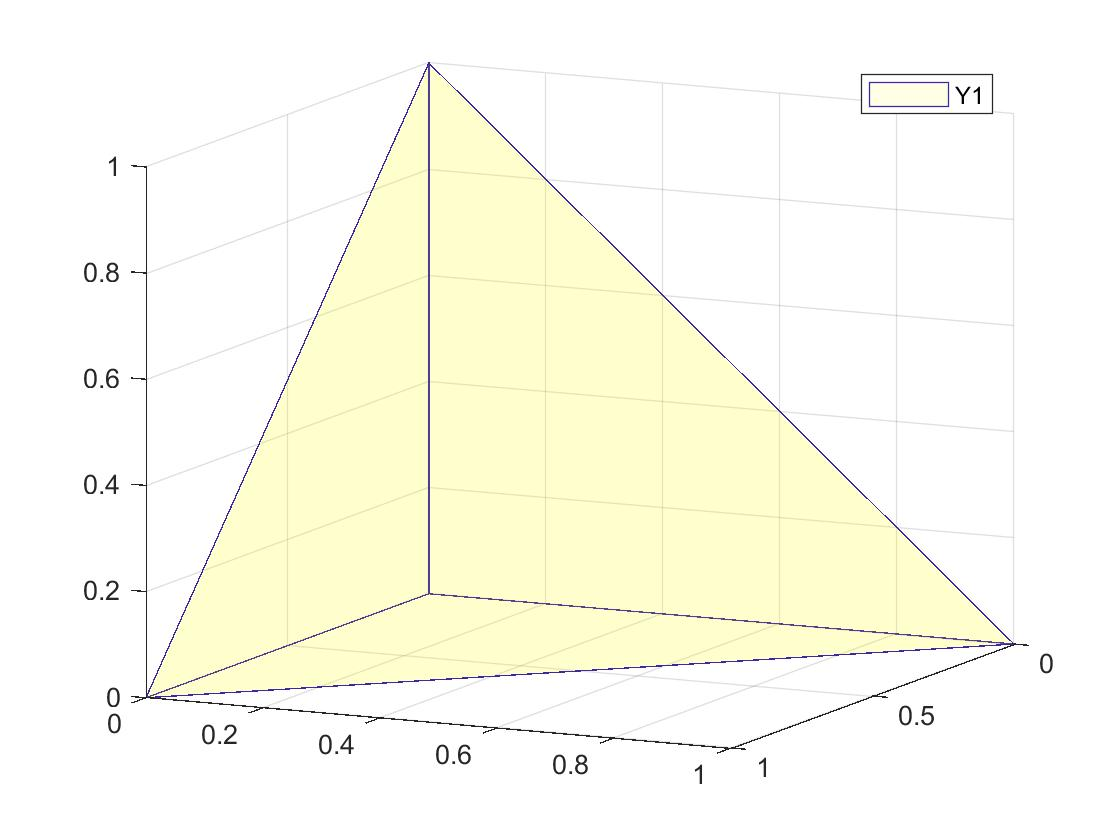
\includegraphics[width=0.45\linewidth]{Simplex1}\\
	\vspace{5mm}
	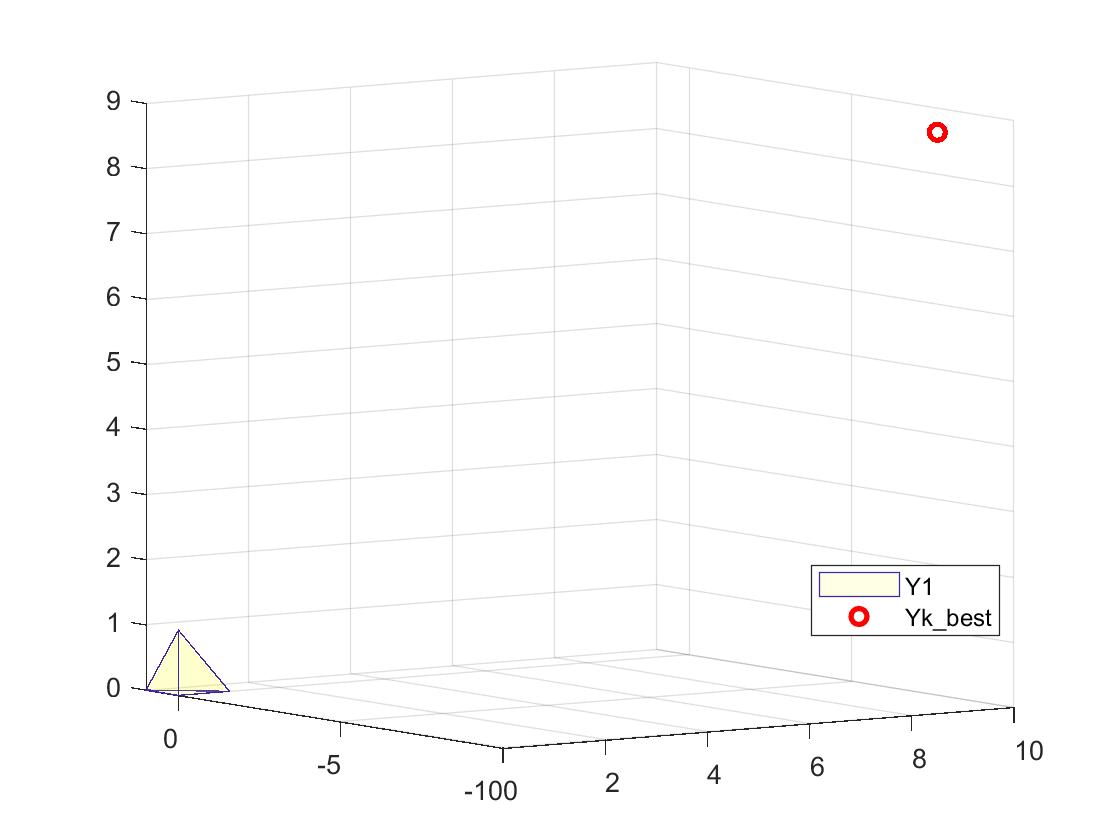
\includegraphics[width=0.45\linewidth]{1aSimplexPlot}
\end{column}
\end{columns}
\end{block}
\end{frame}

\begin{frame}{The Rheology Problem: Solved}
\begin{block}{2.b) New parameters with simplex B}
\begin{columns}
\begin{column}{0.35\linewidth}
	\underline{Input:}\\
	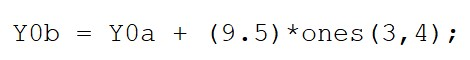
\includegraphics[width=0.75\linewidth]{Y0b}\\
	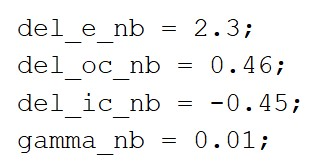
\includegraphics[width=0.45\linewidth]{NewParamsB}\\
	\vspace{0.65cm}
	\underline{Output:}\\
	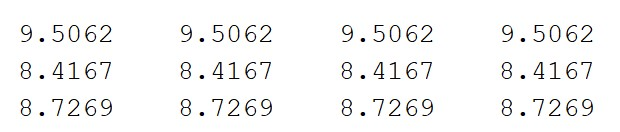
\includegraphics[width=0.95\linewidth]{1bSimplex}
	$$f^k_{best} = 32.7238$$
	\vspace{0.1cm}
\end{column}
\begin{column}{0.63\linewidth}
	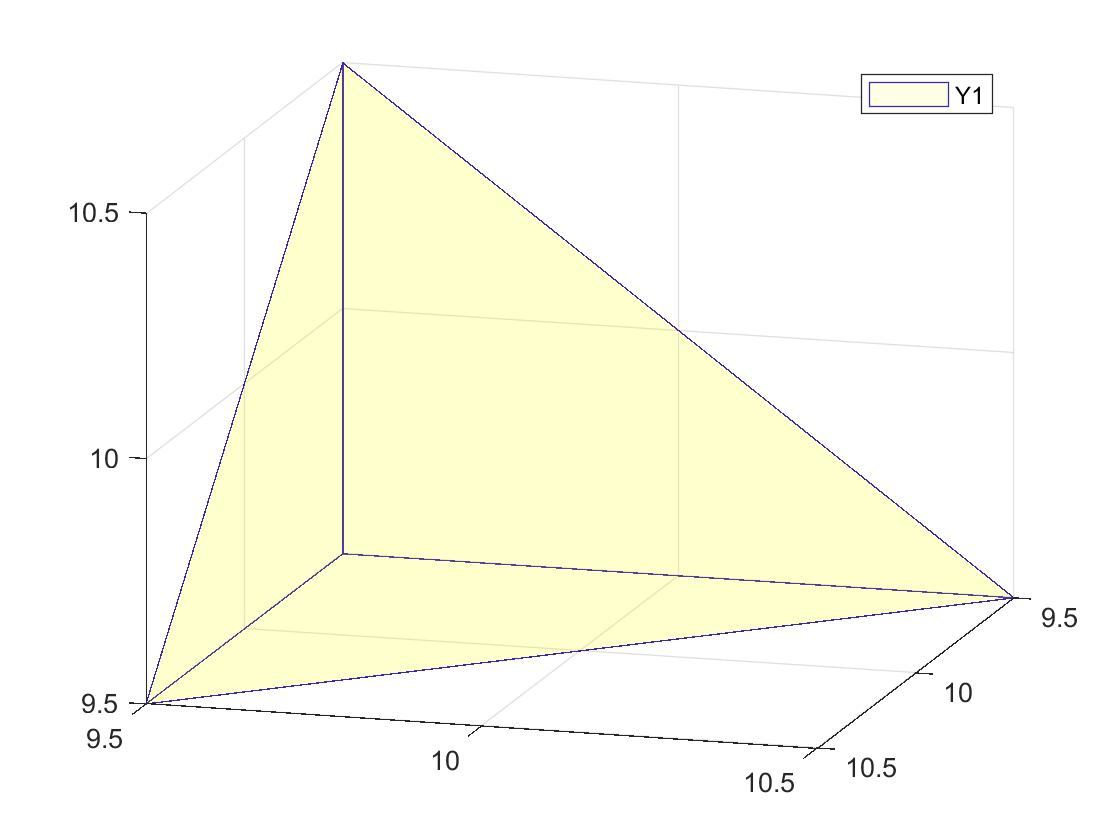
\includegraphics[width=0.45\linewidth]{Simplex2}\\
	\vspace{5mm}
	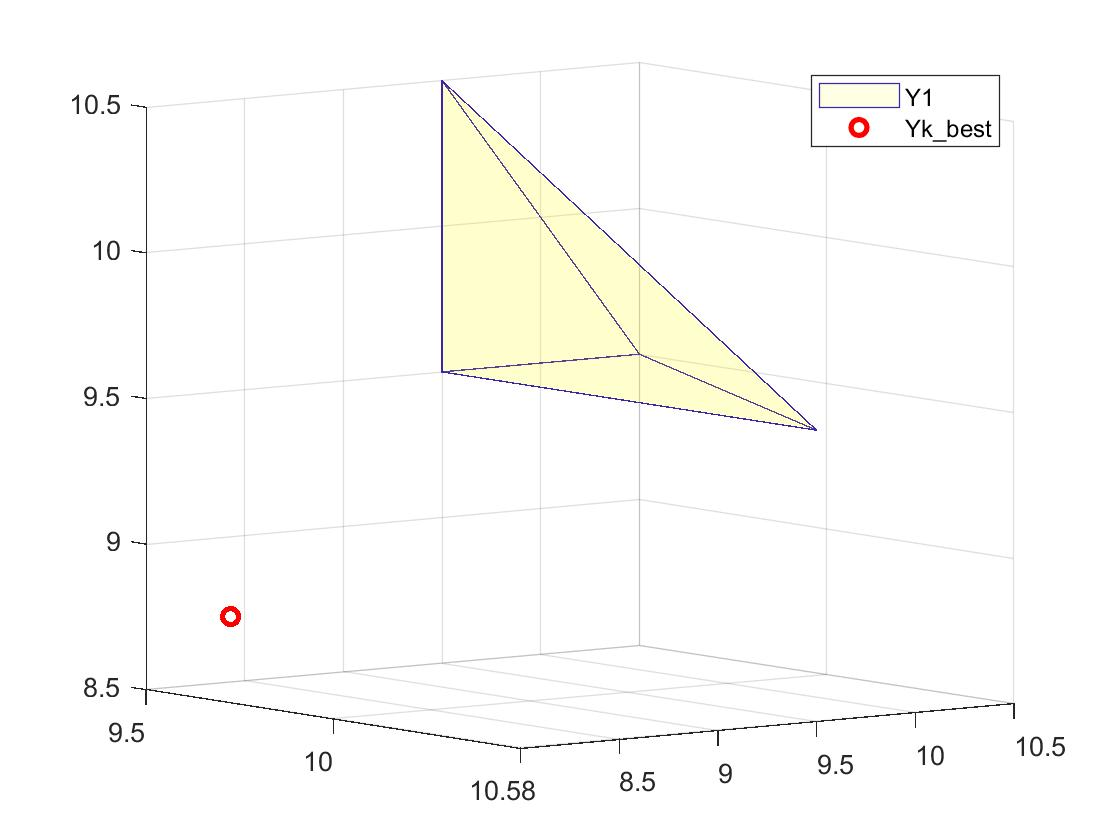
\includegraphics[width=0.45\linewidth]{1bSimplexPlot}
\end{column}
\end{columns}
\end{block}
\end{frame}

\begin{frame}{The Rheology Problem: Solved}
	\centering
	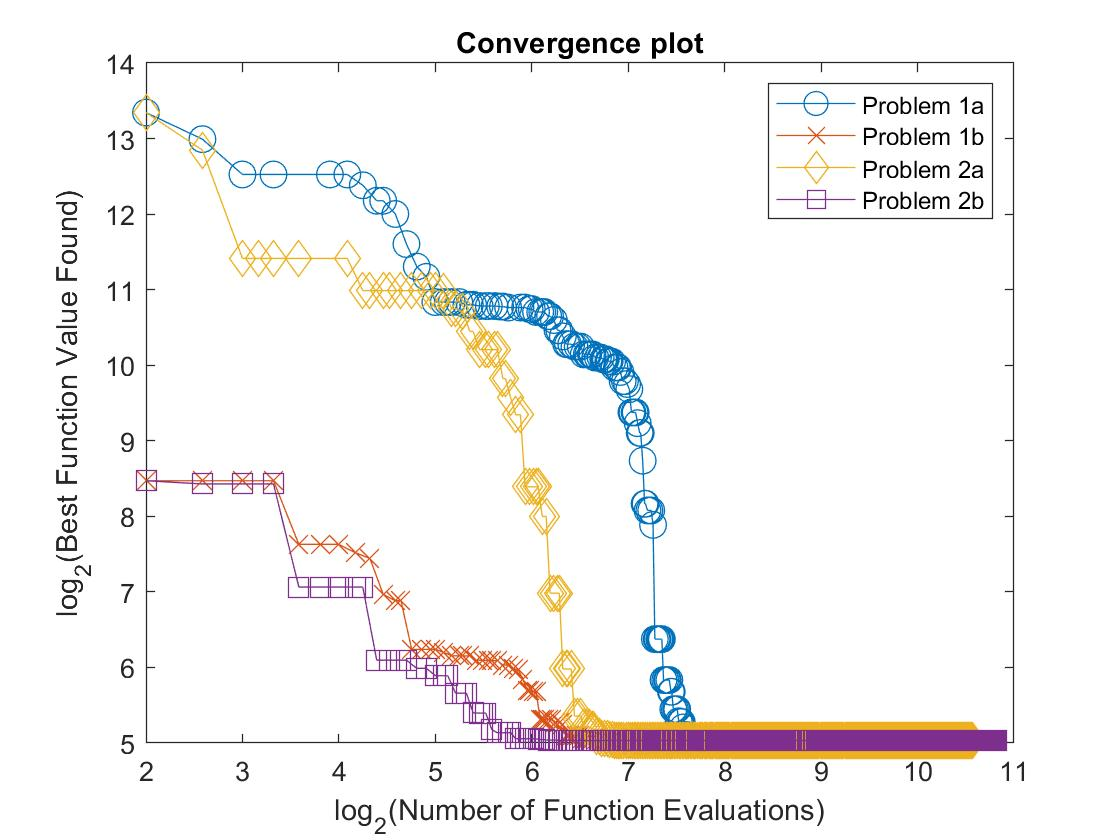
\includegraphics[width=0.85\linewidth]{convergencePlot}
\end{frame}


\end{document}